\documentclass[11pt]{article}

\usepackage{mathptmx}
\usepackage{url}
\usepackage{graphicx}

\newcommand*{\p}[1]{\textup{\texttt{#1}}}
\newcommand*{\ls}{\textsc{LearnSAT}}
\newcommand*{\pl}{\textsc{Prolog}}
\newcommand*{\sw}{\textsc{SWI-Prolog}}
\newcommand*{\dt}{\textsc{dot}}

\textwidth=15cm
\textheight=22.5cm
\topmargin=0pt
\headheight=0pt
\oddsidemargin=1cm
\headsep=0pt
\renewcommand{\baselinestretch}{1.1}
\setlength{\parskip}{0.20\baselineskip plus 1pt minus 1pt}
\parindent=0pt

\author{\bfseries Mordechai (Moti) Ben-Ari\\\url{http: //www.weizmann.ac.il/sci-tea/benari/}}
\title{\bfseries \ls\\\mbox{}\\
\bfseries\large User's Guide\\\mbox{}\\
\bfseries\normalsize Version 1.0.6}

%\date{}
\begin{document}
\maketitle
\thispagestyle{empty}

\vfill

\begin{center}
Copyright \copyright{} 2012 by Mordechai (Moti) Ben-Ari.
\end{center}
This work is licensed under the Creative Commons Attribution-ShareAlike 3.0
License. To view a copy of this license, visit
\url{http://creativecommons.org/licenses/by-sa/3.0/}; or, (b) send a letter
to Creative Commons, 543 Howard Street, 5th Floor, San Francisco,
California, 94105, USA.

\bigskip

 
\begin{center}
The following copyright notice applies to the programs described in this
document:\mbox{}\\\mbox{}\\
Copyright 2012 by Mordechai (Moti) Ben-Ari.
\end{center}

This program is free software; you can redistribute it and/or
modify it under the terms of the GNU General Public License
as published by the Free Software Foundation; either version 2
of the License, or (at your option) any later version.
This program is distributed in the hope that it will be useful
but WITHOUT ANY WARRANTY; without even the implied warranty of
MERCHANTABILITY or FITNESS FOR A PARTICULAR PURPOSE.
See the GNU General Public License for more details.
You should have received a copy of the GNU General Public License
along with this program; if not, write to the Free Software
Foundation, Inc., 59 Temple Place - Suite 330, Boston, MA
02111-1307, USA.

\newpage

\section{Introduction}

\ls{} is a program for learning about SAT solving. It implements the
classic \emph{Davis-Putnam-Logemann-Loveland (DPLL)} algorithm for SAT
solving, together will modern extensions of the algorithm:
\emph{conflict-driven clause learning (CDCL)} and
\emph{non-chronological backtracking (NCB)}.

For a gentle introduction to SAT solvers, see \cite[Chapter~6]{mlcs}.
The comprehensive reference is the \emph{Handbook of Satisfiability}
\cite{SAT}. The algorithms and notation of \ls{} follow \cite{mlm}.

The design of \ls{} is based on the following principles:

\begin{itemize}

\item A very detailed trace of the algorithm's execution can be
displayed. The content of the trace can be set by the user.

\item The \pl{} language is used so that the programs will be concise
and easy to understand. The source code includes extensive comments.
Little knowledge of \pl{} is needed just to run the program.

\item The distribution includes test programs, including those taken
from published descriptions of the algorithms.

\item A utility is provided for converting between sets of clauses
represented as \pl{} terms and those in DIMACS format. While the former
are easier to read, existing examples in DIMACS format can be downloaded
and converted.

\item \ls{} is an open-source project.

\end{itemize}

\section{Downloading}
\ls{} can be downloaded from Google Code at:\footnote{This project
contains an archive of \pl{} programs for the algorithms in my textbook
\emph{Mathematical Logic for Computer Science (Third Edition)}
\cite{mlcs}.}
\begin{center}
\url{http://code.google.com/p/mlcs/}.
\end{center}

Download and open the zip archive \p{learnsat-N.zip}. The \pl{} source
code in the directory \p{src} and the documentation is in the directory
\p{docs}.

The programs were developed using \sw{} Version 6.0.0:
\begin{center}
\url{http://www.swi-prolog.org/}.
\end{center}
The source files use the extension \p{pro} instead of the more usual
\p{pl} to avoid conflict with programs in Perl. During the installation
of \sw{}, if you associate the extension \p{pro} with \sw{}, a
program can be launched by double-clicking on its name in a file list. 


\section{Running \ls}

\subsection{Creating a file to check satisfiability}

To check the satisfiability of a CNF formula, create a \pl{} program
that calls the predicate \p{dpll} with the set of clauses represented as
a list of lists of literals. Here is a program for the pigeon-hole
problem for two holes and three pigeons, where \p{pij} means that pigeon
\p{i} is in hole \p{j}:

\begin{verbatim}
:- use_module(dpll).

hole2 :-
  dpll(
  [
  [p11, p12],   [p21, p22],   [p31, p32],   % Each pigeon in hole 1 or 2 
  [~p11, ~p21], [~p11, ~p31], [~p21, ~p31], % No pair is in hole 1
  [~p12, ~p22], [~p12, ~p32], [~p22, ~p32], % No pair is in hole 2
  ], _).
\end{verbatim}

The result (a satisfying assignment or \p{[]} if unsatisfiable) is
returned as the second argument, but can be left anonymous if only
the trace is of interest.

\subsection{Loading and running a file}

Once this file has been loaded (by double-clicking or by consulting
\p{[pigeon]}), the query \p{hole2} can be run. After the execution
terminates with \p{true} you must press return to get a new prompt. The
output will be a trace of the DPLL algorithm:

\begin{verbatim}
?- hole2.
LearnSAT v1.0.0. Copyright 2012 by Moti Ben-Ari. GNU GPL.
Decision assignment: p11=0
Propagate unit p12 derived from: 1. [p11,p12]
Propagate unit ~p22 derived from: 7. [~p12,~p22]
Propagate unit p21 derived from: 2. [p21,p22]
Propagate unit ~p31 derived from: 6. [~p21,~p31]
Propagate unit p32 derived from: 3. [p31,p32]
Conflict clause: 8. [~p12,~p32]
Decision assignment: p11=1
                ...
Unsatisfiable
Clauses=9, variables=6, units propagated=56, choices=12, conflicts=12

true.
\end{verbatim}

The trace output can be directed to a file:

\begin{verbatim}
hole2_file :- tell('hole2.txt'), hole2, told.
\end{verbatim}

\subsection{Algorithmic modes and display options}

\ls{} can run in one of three modes set by the predicate \p{set\_mode(Mode)}:
\begin{itemize}
\item \p{dpll}: DPLL algorithm (default);
\item \p{cdcl}: DPLL with conflict-directed clause learning;
\item \p{ncb}:  DPLL with CDCL and non-chronological backtracking.
\end{itemize}

The pigeon-hole program runs much more efficiently in \p{cdcl} mode:
\begin{verbatim}
?- set_mode(cdcl).
true.
?- hole2.
                ...
Unsatisfiable:
Statistics: clauses=9, variables=6, units propagated=29, choices=12,
  conflicts=12
\end{verbatim}

\ls{} writes extensive trace output as it executes the algorithms. Each
line starts with a string followed by a colon to make it easy to
postprocess the output. In \p{cdcl} and \p{ncb} modes, the assignments
are written together with their levels in the format \p{p1=0@3} used in
\cite{mlm}.

The content of the trace is controlled using \p{set\_display} and
\p{clear\_display}. The argument to these predicates can be \p{all} or
\p{default} or a single option or a list of options taken from table in
the Appendix. If you need to change the mode and options frequently, you
can write a predicate to do so, or you can change the defaults by
editing the file \p{config.pro}.

\subsection{Online help}

The predicate \p{usage} shows the commands, and the mode and display
arguments.

The version, the default and current mode, and the default and current
display options can be shown by running \p{show\_config}.

\subsection{Implication graphs}\label{s.impl}

\ls{} constructs the implication graph when a conflict clause is
encountered and the graph can be displayed (both the final graph and the
graphs that are incrementally constructed). 

The graph can
also be written to a file in \dt{} format which can be rendered using
\textsc{GraphViz}:\footnote{\url{http://www.graphviz.org/}.}

\begin{verbatim}
dot -Tpng examples-graph-0.dot > examples-graph-0.png
\end{verbatim}
You can choose to label the edges with clause numbers as in \cite{mlm}
or with the clauses themselves.

A script to run \dt{} on all the files for the incremental graphs; for
example, in Windows:
\begin{verbatim}
for %%F in (*.dot) do c:\...\graphviz\bin\dot -Tpng %%F > %%~nF.png
\end{verbatim}

\pagebreak[3]

Here is the graph that was generated by running \ls{} on the example
from \cite{mlm}:
\begin{center}
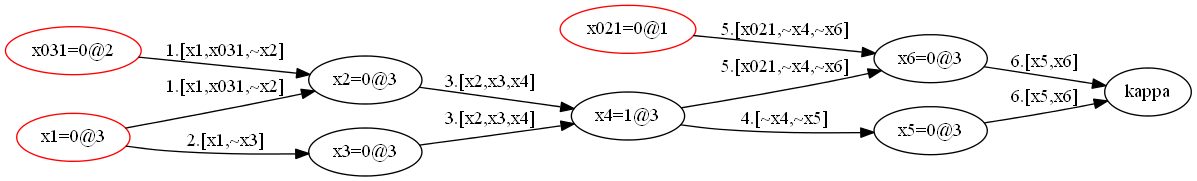
\includegraphics[keepaspectratio=true,width=\textwidth]{graph}
\end{center}
The atom names were modified so that the sequence of assignments
will be as in the paper:
\begin{verbatim}
  1. [x1,x031,~x2]   2. [x1,~x3]         3. [x2,x3,x4]
  4. [~x4,~x5]       5. [x021,~x4,~x6]   6. [x5,x6]
\end{verbatim}

\section{Test programs included in \ls{}}

\begin{itemize}

\item \p{queens.pro}: The four-queens problem as given in
\cite[Section 6.4]{mlcs}.

\item \p{tseitin.pro}: Tseitin clauses for the graphs $K_{2,2}$,
$K_{3,3}$ and the example from \cite[Section 4.5]{mlcs}. These formulas
are unsatisfiable, but for each one a satisfiable variant is given.

\item \p{pigeon.pro} contains the pigeon-hole problem for
two and three holes \cite[Exercise 6.4]{mlcs}.

\item \p{examples.pro} contains examples from papers on SAT
solvers \cite{mz,mlm,ms}.
\end{itemize}


\section{DIMACS transformation}

The predicates in the file \p{dimacs.pro} convert a set of clauses in
\pl{} format (a list of lists of literals) to and from \emph{simplified
DIMACS cnf format} that is used by SAT solvers.
\begin{itemize}
\item \p{to\_dimacs(File, Comment, Clauses)} converts the \pl{}
\p{Clauses} into DIMACS format and writes them to the \p{File} with the
\p{Comment}.
\item \p{from\_dimacs(Predicate, InFile, OutFile)} reads \p{InFile} in
DIMACS format and converts the data into a program written on
\p{OutFile}. \p{Predicate} is the name to be given to the predicate for
running \p{dpll}:
\begin{verbatim}
Predicate :- dpll(List, _).
\end{verbatim}
\end{itemize}

\newpage

\section{Software documentation}

\subsection{Module structure}

The \ls{} software consists of the following source files:\footnote{The
list does not including the test programs and the program for DIMACS
conversion discussed above.}

\begin{itemize}
\item \p{dpll.pro} is the main module for the DPLL algorithms. It is
described in more detail below.

\item \p{io.pro} is a module that writes: (a) assignments; (b) clauses
together with their position numbers from the list of clauses input to
the program; (c) implication graphs.

\item \p{counters.pro} is the module that maintains and displays counters
for units, choices and conflicts, as well as a counter for adding a
number to the file names for implication graphs.

\item \p{display.pro} is the module that writes the explanations using
the predicates \p{display/2},
\p{display/3}, \p{display/4}, whose first argument is a display option
and whose additional arguments supply the data to be displayed.

\item \p{modes.pro} sets, clears and checks the execution mode and the
display options. It also implements \p{usage} and \p{show\_config}. The
dummy display option \p{none} is used to distinguish between the initial
state (no options, so set the default options) and a state where all
options have been cleared.

\item \p{display.pro} is the module that maintains the mode and display
options, and writes the data. The main predicates are \p{display/2},
\p{display/3}, \p{display/4}, whose first argument is a display option
and whose additional arguments supply the data to be displayed. The
dummy display option \p{none} is used to distinguish between the initial
state (no options, so set the default options) and a state where all
options have been cleared.

\item \p{config.pro} is a module that facilitates changing the default
options. It consists of just three facts: \p{version}, \p{default\_mode}
and \p{default\_display}.

\end{itemize}

\subsection{The DPLL algorithm}

The negation operator is defined as \verb+op(610, fy, ~)+ and exported.

The predicate \p{dpll} implements the DPLL algorithm on a set of clauses
represented as a list of lists of literals. It always succeeds,
returning either a list of satisfying assignments or the empty list if
the clauses are unsatisfiable. As part of its initialization, the set of
variables in the clauses is obtained from the list. 

The predicate \p{dpll} invokes \p{dpll1} which is the main recursive
predicate for performing the algorithm. If the set of variables is
empty, the set of clauses is unsatisfiable. Otherwise, \p{dpll1} tries
to perform unit propagation by searching for a unit and then evaluating
the set of clauses. When no more units remain, it chooses a decision
assignment and evaluates the set of clauses.

The predicate \p{ok\_or\_conflict} is called with the result of the
evaluation of unit propagation or the choice of an assignment. If the
result is not a conflict clause, the variable chosen is deleted and
\p{dpll1} is called recursively. If there was a conflict clause, the
implication graph is constructed and a learned clause is generated from
the graph; then \p{ok\_or\_conflict} fails so that backtracking can try
a new assignment.

\subsection{Conflict-directed clause learning and non-chronological backtracking}

See \cite{mlm} for a detailed description of CDCL and NCB.

An \emph{implication graph} represents the result of unit propagation
that causes a conflict. Consider the graph shown in
Section~\ref{s.impl}: There are three source nodes, one for each of the
decision assignments (to \p{x021}, \p{x031}, \p{x1}) that are sufficient
to cause a conflict by unit propagation. The conflict is represented by
the sink node \p{kappa} and the assignments that were forced by unit
propagation are represented by nodes labeled with the assignments. The
edges of the graph are labeled with (the numbers of) the clauses that
are \emph{antecedents} of each node; these are the unit clauses that
forced the assignment labeling that node. There is an edge for each
literal in the unit clause (except the one whose assignment is forced)
and the sources of these edges are the assignments to those literals.
For example, the decision assignments of 0 at levels 2 and 3 to \p{x031}
and \p{x1} cause clause 1 (\verb+[x1, x031, ~x2]+) to become a unit
clause and force the assignment of 0 to \p{x2}.

In \ls{}, the implication graph is built incrementally. Whenever a unit
clause is found, the predicate \p{extend\_graph} is called with the unit
clause, its number (to label the new edges), the assignment it forces
(to create the new target of the edges) and the graph constructed so
far. For each literal (except the one implied), a new edge is created
and when the list of literals has been traversed, the new node is
created. When a conflict is encountered, the \p{kappa} node and its
incoming edges are added and the graph is passed to
\p{compute\_learned\_clause}.

The predicate \p{compute\_learned\_clause} starts with the conflict
clause (the antecedent clause of the \p{kappa} node) as the current
clause and starts resolving. The second clause for each resolution step
is one that clashes with the current clause on a literal that is
assigned at the current level \emph{by unit propagation}. For example,
given the conflict clause \p{[x5,x6]} from the figure, both \p{x5} and
\p{x6} were assigned by unit propagation at this level, so we can
successively resolve \p{[x5,x6]} with the antecedent clauses of the
assignments, namely, \verb+[~x4,~x5]+ and then \verb+[x021,~x4,~x6]+ (or
in the opposite order). The resolution terminates when a \emph{unique
implication point (UIP)} is encountered; this is a clause where only one
literal is assigned at the current level. This clause is the
\emph{learned clause} and is added to the list that is the argument of
the single fact in the database \p{learned}. In the example, the learned
clause is \verb+[x021,~x4]+.

When a learned clause has been obtained, the backtrack level for
non-chronological backtracking is computed. This is the highest level of
an assignment in the learned clause except for the current level. The
level is stored in a dynamic database \p{backtrack} and is used when
choosing an assignment to avoid choosing variables at a lower level than
the backtrack level. In the example, the highest level is 1 where
\p{x021} was assigned.


\pagebreak[4]

\subsection{Auxiliary predicates}

\begin{itemize}

\item \p{evaluate} a set of clauses; returns \p{ok} or \p{conflict}.

\item \p{evaluate\_clause} returns one of \p{satisfied}, \p{unsatisfied},
\p{unit}, \p{unresolved}.

\item \p{choose\_assignment} and \p{choose\_value} return an assignment.
Backtracking is used to return subsequent choices.

The only delicate part is the use of the predicate \emph{Condition}
$\rightarrow$ \emph{Action} with an internal \p{!, fail} to implement
non-chronological backtracing; see the comments and Section~4.7 of the
\sw{} Reference Manual.

\item \p{is\_assigned} checks if a literal is assigned a value
and if so returns that value (0 or 1).

\item \p{resolve} performs resolution on two clauses.

\item \p{literals\_to\_variables} takes a list of literals and returns a
sorted set of the variables corresponding to the literals.

\item \p{to\_variable} returns the variable of a literal and
\p{to\_complement} returns the complement of a literal.

\item \p{to\_assignment} and \p{to\_literal} convert to and from a
literal and an assignment expressed as a term \p{assign(Variable, Value,
Level, Decision)}, where \p{Level} is the level at which the assignment
was made and \p{Decision} is \p{yes} if the assignment was
made as a decision and \p{no} if the assignment was the result of unit
propagation.

\end{itemize}


\bibliographystyle{plain}
\bibliography{learnsat}

\newpage

\appendix
\section{Reference}

\bigskip\bigskip

\begin{center}
\begin{tabular}{|l|l|}
\hline
\multicolumn{2}{|c|}{\textbf{\large Predicates}}\\
\hline
\p{dpll}&Run the DPLL algorithm\\
\p{usage}&Show the predicates, modes and display options \\
\p{show\_config}&Show the current mode and display options\\
\p{set\_display}&Set display options\\
\p{clear\_display}&Clear display options\\
\p{set\_mode}&Set the algorithmic mode\\
\p{to\_dimacs}&Convert from \pl{} term to DIMACS\\
\p{from\_dimacs}&Convert from DIMACS to \pl{} term\\
\hline
\multicolumn{2}{c}{}\\
\hline
\multicolumn{2}{|c|}{\textbf{\large Modes}}\\
\hline
\p{dpll} & DPLL algorithm (default)\\
\p{cdcl} & DPLL with conflict-directed clause learning\\
\p{ncb} &  DPLL with CDCL and non-chronological backtracking\\
\hline
\multicolumn{2}{c}{}\\
\hline
\multicolumn{2}{|c|}{\textbf{\large Display options}}\\
\hline
\p{all}       &  all of the options\\
\p{default}   &  default options (indicated by *)\\
\hline
\p{assignments}& assignments that caused a conflict         \\
\p{backtrack}*&  level of non-chronological backtracking    \\
\p{clauses}   &  clauses to be checked for satisfiability   \\
\p{conflict}* &  conflict clauses                           \\
\p{decision}* &  decision assignments                       \\
\p{evaluate}  &  evaluation of clauses for an assignment    \\
\p{dot}       &  implication graphs in dot format           \\
\p{graph}     &  implication graphs                         \\
\p{incremental}& incremental build of the implication graphs\\
\p{learned}*  &  learned clauses                            \\
\p{literal}   &  literals found assigned during CDCL        \\
\p{partial}   &  partial assignment so far                  \\
\p{resolvent} &  resolvents created during CDCL             \\
\p{result}*   &  result of the algorithm                    \\
\p{skipping}  &  assignments skipped when backtracking      \\
\p{uip}       &  unique implication points                  \\
\p{unit}*     &  unit clauses                               \\
\p{variables} &  variables that are not assigned so far     \\
\hline
\end{tabular}
\end{center}

\end{document}
